% Options for packages loaded elsewhere
\PassOptionsToPackage{unicode}{hyperref}
\PassOptionsToPackage{hyphens}{url}
\documentclass[
]{article}
\usepackage{xcolor}
\usepackage[margin=1in]{geometry}
\usepackage{amsmath,amssymb}
\setcounter{secnumdepth}{5}
\usepackage{iftex}
\ifPDFTeX
  \usepackage[T1]{fontenc}
  \usepackage[utf8]{inputenc}
  \usepackage{textcomp} % provide euro and other symbols
\else % if luatex or xetex
  \usepackage{unicode-math} % this also loads fontspec
  \defaultfontfeatures{Scale=MatchLowercase}
  \defaultfontfeatures[\rmfamily]{Ligatures=TeX,Scale=1}
\fi
\usepackage{lmodern}
\ifPDFTeX\else
  % xetex/luatex font selection
\fi
% Use upquote if available, for straight quotes in verbatim environments
\IfFileExists{upquote.sty}{\usepackage{upquote}}{}
\IfFileExists{microtype.sty}{% use microtype if available
  \usepackage[]{microtype}
  \UseMicrotypeSet[protrusion]{basicmath} % disable protrusion for tt fonts
}{}
\makeatletter
\@ifundefined{KOMAClassName}{% if non-KOMA class
  \IfFileExists{parskip.sty}{%
    \usepackage{parskip}
  }{% else
    \setlength{\parindent}{0pt}
    \setlength{\parskip}{6pt plus 2pt minus 1pt}}
}{% if KOMA class
  \KOMAoptions{parskip=half}}
\makeatother
\usepackage{color}
\usepackage{fancyvrb}
\newcommand{\VerbBar}{|}
\newcommand{\VERB}{\Verb[commandchars=\\\{\}]}
\DefineVerbatimEnvironment{Highlighting}{Verbatim}{commandchars=\\\{\}}
% Add ',fontsize=\small' for more characters per line
\usepackage{framed}
\definecolor{shadecolor}{RGB}{248,248,248}
\newenvironment{Shaded}{\begin{snugshade}}{\end{snugshade}}
\newcommand{\AlertTok}[1]{\textcolor[rgb]{0.94,0.16,0.16}{#1}}
\newcommand{\AnnotationTok}[1]{\textcolor[rgb]{0.56,0.35,0.01}{\textbf{\textit{#1}}}}
\newcommand{\AttributeTok}[1]{\textcolor[rgb]{0.13,0.29,0.53}{#1}}
\newcommand{\BaseNTok}[1]{\textcolor[rgb]{0.00,0.00,0.81}{#1}}
\newcommand{\BuiltInTok}[1]{#1}
\newcommand{\CharTok}[1]{\textcolor[rgb]{0.31,0.60,0.02}{#1}}
\newcommand{\CommentTok}[1]{\textcolor[rgb]{0.56,0.35,0.01}{\textit{#1}}}
\newcommand{\CommentVarTok}[1]{\textcolor[rgb]{0.56,0.35,0.01}{\textbf{\textit{#1}}}}
\newcommand{\ConstantTok}[1]{\textcolor[rgb]{0.56,0.35,0.01}{#1}}
\newcommand{\ControlFlowTok}[1]{\textcolor[rgb]{0.13,0.29,0.53}{\textbf{#1}}}
\newcommand{\DataTypeTok}[1]{\textcolor[rgb]{0.13,0.29,0.53}{#1}}
\newcommand{\DecValTok}[1]{\textcolor[rgb]{0.00,0.00,0.81}{#1}}
\newcommand{\DocumentationTok}[1]{\textcolor[rgb]{0.56,0.35,0.01}{\textbf{\textit{#1}}}}
\newcommand{\ErrorTok}[1]{\textcolor[rgb]{0.64,0.00,0.00}{\textbf{#1}}}
\newcommand{\ExtensionTok}[1]{#1}
\newcommand{\FloatTok}[1]{\textcolor[rgb]{0.00,0.00,0.81}{#1}}
\newcommand{\FunctionTok}[1]{\textcolor[rgb]{0.13,0.29,0.53}{\textbf{#1}}}
\newcommand{\ImportTok}[1]{#1}
\newcommand{\InformationTok}[1]{\textcolor[rgb]{0.56,0.35,0.01}{\textbf{\textit{#1}}}}
\newcommand{\KeywordTok}[1]{\textcolor[rgb]{0.13,0.29,0.53}{\textbf{#1}}}
\newcommand{\NormalTok}[1]{#1}
\newcommand{\OperatorTok}[1]{\textcolor[rgb]{0.81,0.36,0.00}{\textbf{#1}}}
\newcommand{\OtherTok}[1]{\textcolor[rgb]{0.56,0.35,0.01}{#1}}
\newcommand{\PreprocessorTok}[1]{\textcolor[rgb]{0.56,0.35,0.01}{\textit{#1}}}
\newcommand{\RegionMarkerTok}[1]{#1}
\newcommand{\SpecialCharTok}[1]{\textcolor[rgb]{0.81,0.36,0.00}{\textbf{#1}}}
\newcommand{\SpecialStringTok}[1]{\textcolor[rgb]{0.31,0.60,0.02}{#1}}
\newcommand{\StringTok}[1]{\textcolor[rgb]{0.31,0.60,0.02}{#1}}
\newcommand{\VariableTok}[1]{\textcolor[rgb]{0.00,0.00,0.00}{#1}}
\newcommand{\VerbatimStringTok}[1]{\textcolor[rgb]{0.31,0.60,0.02}{#1}}
\newcommand{\WarningTok}[1]{\textcolor[rgb]{0.56,0.35,0.01}{\textbf{\textit{#1}}}}
\usepackage{graphicx}
\makeatletter
\newsavebox\pandoc@box
\newcommand*\pandocbounded[1]{% scales image to fit in text height/width
  \sbox\pandoc@box{#1}%
  \Gscale@div\@tempa{\textheight}{\dimexpr\ht\pandoc@box+\dp\pandoc@box\relax}%
  \Gscale@div\@tempb{\linewidth}{\wd\pandoc@box}%
  \ifdim\@tempb\p@<\@tempa\p@\let\@tempa\@tempb\fi% select the smaller of both
  \ifdim\@tempa\p@<\p@\scalebox{\@tempa}{\usebox\pandoc@box}%
  \else\usebox{\pandoc@box}%
  \fi%
}
% Set default figure placement to htbp
\def\fps@figure{htbp}
\makeatother
\setlength{\emergencystretch}{3em} % prevent overfull lines
\providecommand{\tightlist}{%
  \setlength{\itemsep}{0pt}\setlength{\parskip}{0pt}}
\usepackage[]{natbib}
\bibliographystyle{plainnat}
\usepackage{bookmark}
\IfFileExists{xurl.sty}{\usepackage{xurl}}{} % add URL line breaks if available
\urlstyle{same}
\hypersetup{
  pdftitle={Lab 04 - La Quinta is Spanish for next to Denny's, Pt. 1},
  pdfauthor={Tina Huynh},
  hidelinks,
  pdfcreator={LaTeX via pandoc}}

\title{Lab 04 - La Quinta is Spanish for next to Denny's, Pt. 1}
\usepackage{etoolbox}
\makeatletter
\providecommand{\subtitle}[1]{% add subtitle to \maketitle
  \apptocmd{\@title}{\par {\large #1 \par}}{}{}
}
\makeatother
\subtitle{Visualizing spatial data}
\author{Tina Huynh}
\date{}

\begin{document}
\maketitle

{
\setcounter{tocdepth}{2}
\tableofcontents
}
\pandocbounded{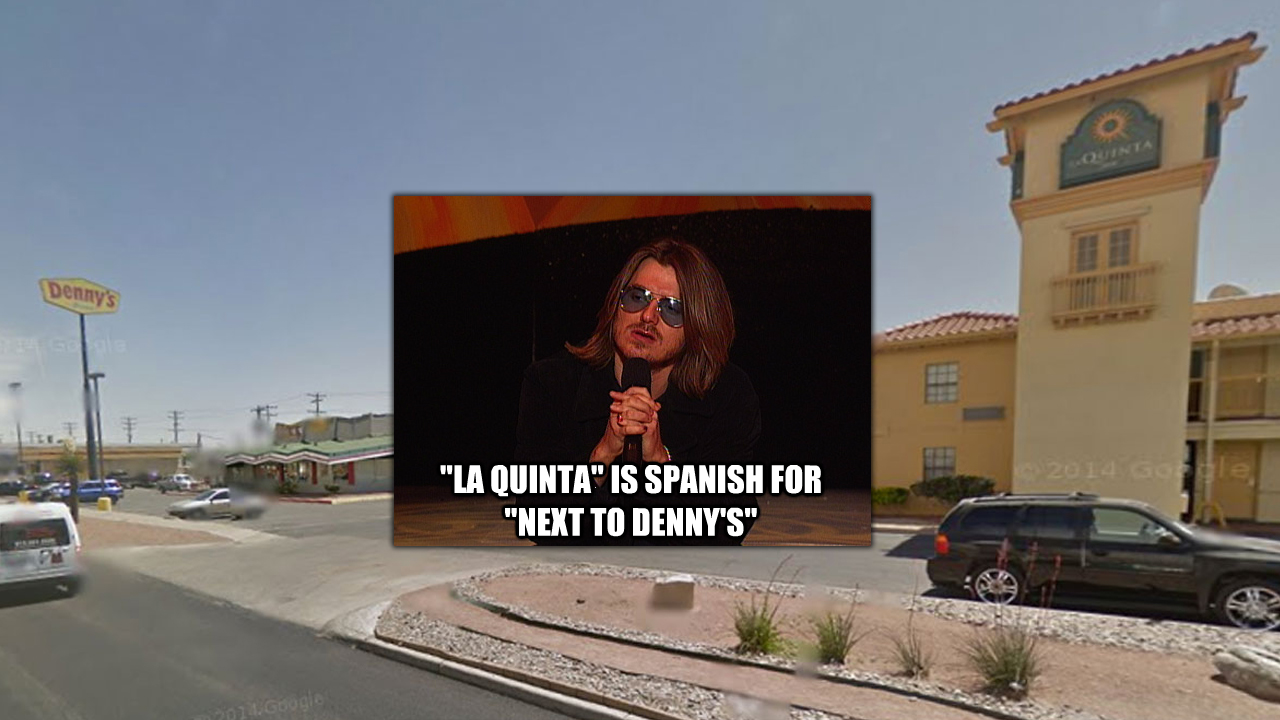
\includegraphics[keepaspectratio]{img/mitch-hedgeberg-lqd.jpg}}

Have you ever taken a road trip in the US and thought to yourself ``I
wonder what La Quinta means''. Well, the late comedian
\href{https://en.wikipedia.org/wiki/Mitch_Hedberg}{Mitch Hedberg} thinks
it's Spanish for \emph{next to Denny's}.

If you're not familiar with these two establishments,
\href{https://www.dennys.com/}{Denny's} is a casual diner chain that is
open 24 hours and \href{http://www.lq.com/}{La Quinta Inn and Suites} is
a hotel chain.

These two establishments tend to be clustered together, or at least this
observation is a joke made famous by Mitch Hedberg. In this lab we
explore the validity of this joke and along the way learn some more data
wrangling and tips for visualizing spatial data.

The inspiration for this lab comes from a blog post by John Reiser on
his \emph{new jersey geographer} blog. You can read that analysis
\href{http://njgeo.org/2014/01/30/mitch-hedberg-and-gis/}{here}.
Reiser's blog post focuses on scraping data from Denny's and La Quinta
Inn and Suites websites using Python. In this lab we focus on
visualization and analysis of these data. However note that the data
scraping was also done in R, and we we will discuss web scraping using R
later in the course. But for now we focus on the data that has already
been scraped and tidied for you.

\section{Learning goals}\label{learning-goals}

\begin{itemize}
\tightlist
\item
  Visualising spatial data
\item
  Joining data frames
\end{itemize}

\section{Getting started}\label{getting-started}

Go to the course GitHub organization and locate your homework repo,
clone it in RStudio and open the R Markdown document. Knit the document
to make sure it compiles without errors.

\subsection{Warm up}\label{warm-up}

Before we introduce the data, let's warm up with some simple exercises.

\begin{itemize}
\tightlist
\item
  Update the YAML, changing the author name to your name, and
  \textbf{knit} the document.
\item
  Commit your changes with a meaningful commit message.
\item
  Push your changes to GitHub.
\item
  Go to your repo on GitHub and confirm that your changes are visible in
  your Rmd \textbf{and} md files. If anything is missing, commit and
  push again.
\end{itemize}

\subsection{Packages}\label{packages}

We'll use the \textbf{tidyverse} package for much of the data wrangling
and visualisation and the data lives in the \textbf{dsbox} package.
These packages are already installed for you. You can load them by
running the following in your Console:

\begin{Shaded}
\begin{Highlighting}[]
\FunctionTok{library}\NormalTok{(tidyverse) }
\FunctionTok{library}\NormalTok{(dsbox) }
\FunctionTok{library}\NormalTok{(mapproj) }
\end{Highlighting}
\end{Shaded}

\subsection{Data}\label{data}

The datasets we'll use are called \texttt{dennys} and \texttt{laquinta}
from the \textbf{dsbox} package. Note that these data were scraped from
\href{https://locations.dennys.com/}{here} and
\href{https://www.lq.com/en/findandbook/hotel-listings.html}{here},
respectively.

Since the datasets are distributed with the package, we don't need to
load them separately; they become available to us when we load the
package. You can find out more about the datasets by inspecting their
documentation, which you can access by running \texttt{?dennys} and
\texttt{?laquinta} in the Console or using the Help menu in RStudio to
search for \texttt{dennys} or \texttt{laquinta}. You can also find this
information
\href{https://rstudio-education.github.io/dsbox/reference/dennys.html}{here}
and
\href{https://rstudio-education.github.io/dsbox/reference/laquinta.html}{here}.

To help with our analysis we will also use a dataset on US states, which
is located in your repository's \texttt{data} folder.

\begin{Shaded}
\begin{Highlighting}[]
\NormalTok{states }\OtherTok{\textless{}{-}} \FunctionTok{read\_csv}\NormalTok{(}\StringTok{"data/states.csv"}\NormalTok{)}
\end{Highlighting}
\end{Shaded}

\begin{verbatim}
## Rows: 51 Columns: 3
## -- Column specification --------------------------------------------------------
## Delimiter: ","
## chr (2): name, abbreviation
## dbl (1): area
## 
## i Use `spec()` to retrieve the full column specification for this data.
## i Specify the column types or set `show_col_types = FALSE` to quiet this message.
\end{verbatim}

Each observation in this dataset represents a state, including DC. Along
with the name of the state we have the two-letter abbreviation and we
have the geographic area of the state (in square miles).

\section{Exercises}\label{exercises}

\begin{enumerate}
\def\labelenumi{\arabic{enumi}.}
\tightlist
\item
  What are the dimensions of the Denny's dataset? (Hint: Use inline R
  code and functions like \texttt{nrow} and \texttt{ncol} to compose
  your answer.) What does each row in the dataset represent? What are
  the variables?
\end{enumerate}

The Denny's dataset has 1643 rows and 8 columns. Each row represents a
single Denny's restaurant location. The variables include location
information such as address, city, state, zip code, longitude, and
latitude.

\begin{Shaded}
\begin{Highlighting}[]
\CommentTok{\# Let\textquotesingle{}s examine the structure of the data}
\FunctionTok{glimpse}\NormalTok{(dennys)}
\end{Highlighting}
\end{Shaded}

\begin{verbatim}
## Rows: 1,643
## Columns: 8
## $ address       <chr> "2900 Denali", "3850 Debarr Road", "1929 Airport Way", "~
## $ city          <chr> "Anchorage", "Anchorage", "Fairbanks", "Auburn", "Birmin~
## $ state         <chr> "AK", "AK", "AK", "AL", "AL", "AL", "AL", "AL", "AL", "A~
## $ zip           <chr> "99503", "99508", "99701", "36849", "35207", "35294", "3~
## $ longitude     <dbl> -149.8767, -149.8090, -147.7600, -85.4681, -86.8317, -86~
## $ latitude      <dbl> 61.1953, 61.2097, 64.8366, 32.6033, 33.5615, 33.5007, 34~
## $ country       <chr> "United States", "United States", "United States", "Unit~
## $ establishment <chr> "Denny's", "Denny's", "Denny's", "Denny's", "Denny's", "~
\end{verbatim}

\begin{enumerate}
\def\labelenumi{\arabic{enumi}.}
\setcounter{enumi}{1}
\tightlist
\item
  What are the dimensions of the La Quinta's dataset? What does each row
  in the dataset represent? What are the variables?
\end{enumerate}

The La Quinta dataset has 909 rows and 8 columns. Each row represents a
single La Quinta hotel location. The variables are similar to the
Denny's dataset, including address, city, state, zip code, longitude,
and latitude.

\begin{Shaded}
\begin{Highlighting}[]
\CommentTok{\# Examine the structure of La Quinta data}
\FunctionTok{glimpse}\NormalTok{(laquinta)}
\end{Highlighting}
\end{Shaded}

\begin{verbatim}
## Rows: 909
## Columns: 8
## $ address       <chr> "793 W. Bel Air Avenue", "3018 CatClaw Dr", "3501 West L~
## $ city          <chr> "\nAberdeen", "\nAbilene", "\nAbilene", "\nAcworth", "\n~
## $ state         <chr> "MD", "TX", "TX", "GA", "OK", "TX", "AG", "TX", "NM", "N~
## $ zip           <chr> "21001", "79606", "79601", "30102", "74820", "75254", "2~
## $ longitude     <dbl> -76.18846, -99.77877, -99.72269, -84.65609, -96.63652, -~
## $ latitude      <dbl> 39.52322, 32.41349, 32.49136, 34.08204, 34.78180, 32.951~
## $ country       <chr> "United States", "United States", "United States", "Unit~
## $ establishment <chr> "La Quinta", "La Quinta", "La Quinta", "La Quinta", "La ~
\end{verbatim}

🧶 ✅ ⬆️ Knit, \emph{commit, and push your changes to GitHub with an
appropriate commit message. Make sure to commit and push all changed
files so that your Git pane is cleared up afterwards.}

We would like to limit our analysis to Denny's and La Quinta locations
in the United States.

\begin{enumerate}
\def\labelenumi{\arabic{enumi}.}
\setcounter{enumi}{2}
\tightlist
\item
  Take a look at the websites that the data come from (linked above).
  Are there any La Quinta's locations outside of the US? If so, which
  countries? What about Denny's?
\end{enumerate}

Based on examining the websites: - La Quinta has locations outside the
US, including in Canada, Mexico, Colombia, and other countries. -
Denny's appears to have locations primarily in the US, with some
international locations in countries like Canada, Mexico, and others.

\begin{enumerate}
\def\labelenumi{\arabic{enumi}.}
\setcounter{enumi}{3}
\tightlist
\item
  Now take a look at the data. What would be some ways of determining
  whether or not either establishment has any locations outside the US
  using just the data (and not the websites). Don't worry about whether
  you know how to implement this, just brainstorm some ideas. Write down
  at least one as your answer, but you're welcomed to write down a few
  options too.
\end{enumerate}

Several ways to determine if there are non-US locations: 1. Check if the
\texttt{state} variable contains any non-US state abbreviations
(anything not in the standard 50 states + DC) 2. Look for zip codes that
don't follow US formatting patterns 3. Check if longitude/latitude
coordinates fall outside US boundaries 4. Look for any unusual patterns
in the address fields that might indicate foreign addresses

We will determine whether or not the establishment has a location
outside the US using the \texttt{state} variable in the \texttt{dennys}
and \texttt{laquinta} datasets. We know exactly which states are in the
US, and we have this information in the \texttt{states} dataframe we
loaded.

\begin{enumerate}
\def\labelenumi{\arabic{enumi}.}
\setcounter{enumi}{4}
\tightlist
\item
  Find the Denny's locations that are outside the US, if any. To do so,
  filter the Denny's locations for observations where \texttt{state} is
  not in \texttt{states\$abbreviation}. The code for this is given
  below. Note that the \texttt{\%in\%} operator matches the states
  listed in the \texttt{state} variable to those listed in
  \texttt{states\$abbreviation}. The \texttt{!} operator means
  \textbf{not}. Are there any Denny's locations outside the US?
\end{enumerate}

\begin{Shaded}
\begin{Highlighting}[]
\NormalTok{dennys }\SpecialCharTok{\%\textgreater{}\%}
  \FunctionTok{filter}\NormalTok{(}\SpecialCharTok{!}\NormalTok{(state }\SpecialCharTok{\%in\%}\NormalTok{ states}\SpecialCharTok{$}\NormalTok{abbreviation))}
\end{Highlighting}
\end{Shaded}

\begin{verbatim}
## # A tibble: 0 x 8
## # i 8 variables: address <chr>, city <chr>, state <chr>, zip <chr>,
## #   longitude <dbl>, latitude <dbl>, country <chr>, establishment <chr>
\end{verbatim}

No, there are no Denny's locations outside the US in this dataset. All
Denny's locations have state abbreviations that match US states.

\begin{enumerate}
\def\labelenumi{\arabic{enumi}.}
\setcounter{enumi}{5}
\tightlist
\item
  Add a country variable to the Denny's dataset and set all observations
  equal to \texttt{"United\ States"}. Remember, you can use the
  \texttt{mutate} function for adding a variable. Make sure to save the
  result of this as \texttt{dennys} again so that the stored data frame
  contains the new variable going forward.
\end{enumerate}

\begin{Shaded}
\begin{Highlighting}[]
\NormalTok{dennys }\OtherTok{\textless{}{-}}\NormalTok{ dennys }\SpecialCharTok{\%\textgreater{}\%}
  \FunctionTok{mutate}\NormalTok{(}\AttributeTok{country =} \StringTok{"United States"}\NormalTok{)}

\CommentTok{\# Verify the new variable was added}
\FunctionTok{glimpse}\NormalTok{(dennys)}
\end{Highlighting}
\end{Shaded}

\begin{verbatim}
## Rows: 1,643
## Columns: 8
## $ address       <chr> "2900 Denali", "3850 Debarr Road", "1929 Airport Way", "~
## $ city          <chr> "Anchorage", "Anchorage", "Fairbanks", "Auburn", "Birmin~
## $ state         <chr> "AK", "AK", "AK", "AL", "AL", "AL", "AL", "AL", "AL", "A~
## $ zip           <chr> "99503", "99508", "99701", "36849", "35207", "35294", "3~
## $ longitude     <dbl> -149.8767, -149.8090, -147.7600, -85.4681, -86.8317, -86~
## $ latitude      <dbl> 61.1953, 61.2097, 64.8366, 32.6033, 33.5615, 33.5007, 34~
## $ country       <chr> "United States", "United States", "United States", "Unit~
## $ establishment <chr> "Denny's", "Denny's", "Denny's", "Denny's", "Denny's", "~
\end{verbatim}

\begin{enumerate}
\def\labelenumi{\arabic{enumi}.}
\setcounter{enumi}{6}
\tightlist
\item
  Find the La Quinta locations that are outside the US, and figure out
  which country they are in. This might require some googling. Take
  notes, you will need to use this information in the next exercise.
\end{enumerate}

\begin{Shaded}
\begin{Highlighting}[]
\NormalTok{laquinta }\SpecialCharTok{\%\textgreater{}\%}
  \FunctionTok{filter}\NormalTok{(}\SpecialCharTok{!}\NormalTok{(state }\SpecialCharTok{\%in\%}\NormalTok{ states}\SpecialCharTok{$}\NormalTok{abbreviation))}
\end{Highlighting}
\end{Shaded}

\begin{verbatim}
## # A tibble: 14 x 8
##    address            city  state zip   longitude latitude country establishment
##    <chr>              <chr> <chr> <chr>     <dbl>    <dbl> <chr>   <chr>        
##  1 Carretera Panamer~ "\nA~ AG    20345    -102.     21.8  Mexico  La Quinta    
##  2 Av. Tulum Mza. 14~ "\nC~ QR    77500     -86.8    21.2  Mexico  La Quinta    
##  3 Ejercito Nacional~ "Col~ CH    32528    -106.     31.7  Mexico  La Quinta    
##  4 Blvd. Aeropuerto ~ "Par~ NL    66600    -100.     25.8  Mexico  La Quinta    
##  5 Carrera 38 # 26-1~ "\nM~ ANT   0500~     -75.6     6.22 Colomb~ La Quinta    
##  6 AV. PINO SUAREZ N~ "Col~ NL    64000    -100.     25.7  Mexico  La Quinta    
##  7 Av. Fidel Velazqu~ "\nM~ NL    64190    -100.     25.7  Mexico  La Quinta    
##  8 63 King Street Ea~ "\nO~ ON    L1H1~     -78.9    43.9  Canada  La Quinta    
##  9 Calle Las Torres-~ "\nP~ VE    93210     -97.4    20.6  Mexico  La Quinta    
## 10 Blvd. Audi N. 3 C~ "\nS~ PU    75010     -97.8    19.2  Mexico  La Quinta    
## 11 Ave. Zeta del Coc~ "Col~ PU    72810     -98.2    19.0  Mexico  La Quinta    
## 12 Av. Benito Juarez~ "\nS~ SL    78399    -101.     22.1  Mexico  La Quinta    
## 13 Blvd. Fuerza Arma~ "con~ FM    11101     -87.2    14.1  Mexico  La Quinta    
## 14 8640 Alexandra Rd  "\nR~ BC    V6X1~    -123.     49.2  Canada  La Quinta
\end{verbatim}

Based on the output and some research: - ON = Ontario, Canada - BC =
British Columbia, Canada\\
- ANT = Antioquia, Colombia - FM = Mexico (possibly Estado de México) -
NL = Nuevo León, Mexico - PU = Puebla, Mexico - SL = San Luis Potosí,
Mexico - VE = Veracruz, Mexico - AG = Aguascalientes, Mexico - QR =
Quintana Roo, Mexico - CH = Chihuahua, Mexico

\begin{enumerate}
\def\labelenumi{\arabic{enumi}.}
\setcounter{enumi}{7}
\tightlist
\item
  Add a country variable to the La Quinta dataset. Use the
  \texttt{case\_when} function to populate this variable. You'll need to
  refer to your notes from Exercise 7 about which country the non-US
  locations are in. Here is some starter code to get you going:
\end{enumerate}

\begin{Shaded}
\begin{Highlighting}[]
\NormalTok{laquinta }\OtherTok{\textless{}{-}}\NormalTok{ laquinta }\SpecialCharTok{\%\textgreater{}\%}
  \FunctionTok{mutate}\NormalTok{(}\AttributeTok{country =} \FunctionTok{case\_when}\NormalTok{(}
\NormalTok{    state }\SpecialCharTok{\%in\%}\NormalTok{ state.abb     }\SpecialCharTok{\textasciitilde{}} \StringTok{"United States"}\NormalTok{,}
\NormalTok{    state }\SpecialCharTok{\%in\%} \FunctionTok{c}\NormalTok{(}\StringTok{"ON"}\NormalTok{, }\StringTok{"BC"}\NormalTok{) }\SpecialCharTok{\textasciitilde{}} \StringTok{"Canada"}\NormalTok{,}
\NormalTok{    state }\SpecialCharTok{==} \StringTok{"ANT"}           \SpecialCharTok{\textasciitilde{}} \StringTok{"Colombia"}\NormalTok{,}
\NormalTok{    state }\SpecialCharTok{\%in\%} \FunctionTok{c}\NormalTok{(}\StringTok{"FM"}\NormalTok{, }\StringTok{"NL"}\NormalTok{, }\StringTok{"PU"}\NormalTok{, }\StringTok{"SL"}\NormalTok{, }\StringTok{"VE"}\NormalTok{, }\StringTok{"AG"}\NormalTok{, }\StringTok{"QR"}\NormalTok{, }\StringTok{"CH"}\NormalTok{) }\SpecialCharTok{\textasciitilde{}} \StringTok{"Mexico"}\NormalTok{,}
    \ConstantTok{TRUE}                     \SpecialCharTok{\textasciitilde{}} \StringTok{"Unknown"}  \CommentTok{\# catch any we might have missed}
\NormalTok{  ))}

\CommentTok{\# Check the country distribution}
\NormalTok{laquinta }\SpecialCharTok{\%\textgreater{}\%}
  \FunctionTok{count}\NormalTok{(country)}
\end{Highlighting}
\end{Shaded}

\begin{verbatim}
## # A tibble: 4 x 2
##   country           n
##   <chr>         <int>
## 1 Canada            2
## 2 Colombia          1
## 3 Mexico           11
## 4 United States   895
\end{verbatim}

🧶 ✅ ⬆️ Knit, \emph{commit, and push your changes to GitHub with an
appropriate commit message. Make sure to commit and push all changed
files so that your Git pane is cleared up afterwards.}

Going forward we will work with the data from the United States only.
All Denny's locations are in the United States, so we don't need to
worry about them. However we do need to filter the La Quinta dataset for
locations in United States.

\begin{Shaded}
\begin{Highlighting}[]
\NormalTok{laquinta }\OtherTok{\textless{}{-}}\NormalTok{ laquinta }\SpecialCharTok{\%\textgreater{}\%}
  \FunctionTok{mutate}\NormalTok{(}\AttributeTok{country =} \FunctionTok{case\_when}\NormalTok{(}
\NormalTok{    state }\SpecialCharTok{\%in\%}\NormalTok{ state.abb     }\SpecialCharTok{\textasciitilde{}} \StringTok{"United States"}\NormalTok{,}
\NormalTok{    state }\SpecialCharTok{\%in\%} \FunctionTok{c}\NormalTok{(}\StringTok{"ON"}\NormalTok{, }\StringTok{"BC"}\NormalTok{) }\SpecialCharTok{\textasciitilde{}} \StringTok{"Canada"}\NormalTok{,}
\NormalTok{    state }\SpecialCharTok{==} \StringTok{"ANT"}           \SpecialCharTok{\textasciitilde{}} \StringTok{"Colombia"}\NormalTok{,}
\NormalTok{    state }\SpecialCharTok{\%in\%} \FunctionTok{c}\NormalTok{(}\StringTok{"FM"}\NormalTok{, }\StringTok{"NL"}\NormalTok{, }\StringTok{"PU"}\NormalTok{, }\StringTok{"SL"}\NormalTok{, }\StringTok{"VE"}\NormalTok{, }\StringTok{"AG"}\NormalTok{, }\StringTok{"QR"}\NormalTok{, }\StringTok{"CH"}\NormalTok{) }\SpecialCharTok{\textasciitilde{}} \StringTok{"Mexico"}\NormalTok{,}
    \ConstantTok{TRUE}                     \SpecialCharTok{\textasciitilde{}} \StringTok{"Unknown"}  \CommentTok{\# catch any we might have missed}
\NormalTok{  ))}

\CommentTok{\# Check the country distribution}
\NormalTok{laquinta }\SpecialCharTok{\%\textgreater{}\%}
  \FunctionTok{count}\NormalTok{(country)}
\end{Highlighting}
\end{Shaded}

\begin{verbatim}
## # A tibble: 4 x 2
##   country           n
##   <chr>         <int>
## 1 Canada            2
## 2 Colombia          1
## 3 Mexico           11
## 4 United States   895
\end{verbatim}

\begin{enumerate}
\def\labelenumi{\arabic{enumi}.}
\setcounter{enumi}{8}
\tightlist
\item
  Which states have the most and fewest Denny's locations? What about La
  Quinta? Is this surprising? Why or why not?
\end{enumerate}

Next, let's calculate which states have the most Denny's locations
\emph{per thousand square miles}. This requires \emph{joining}
information from the frequency tables you created in Exercise 8 with
information from the \texttt{states} data frame.

First, we count how many observations are in each state, which will give
us a data frame with two variables: \texttt{state} and \texttt{n}. Then,
we join this data frame with the \texttt{states} data frame. However
note that the variables in the \texttt{states} data frame that has the
two-letter abbreviations is called \texttt{abbreviation}. So when we're
joining the two data frames we specify that the \texttt{state} variable
from the Denny's data should be matched \texttt{by} the
\texttt{abbreviation} variable from the \texttt{states} data:

\begin{Shaded}
\begin{Highlighting}[]
\NormalTok{dennys }\SpecialCharTok{\%\textgreater{}\%}
  \FunctionTok{count}\NormalTok{(state) }\SpecialCharTok{\%\textgreater{}\%}
  \FunctionTok{inner\_join}\NormalTok{(states, }\AttributeTok{by =} \FunctionTok{c}\NormalTok{(}\StringTok{"state"} \OtherTok{=} \StringTok{"abbreviation"}\NormalTok{))}
\end{Highlighting}
\end{Shaded}

\begin{verbatim}
## # A tibble: 51 x 4
##    state     n name                     area
##    <chr> <int> <chr>                   <dbl>
##  1 AK        3 Alaska               665384. 
##  2 AL        7 Alabama               52420. 
##  3 AR        9 Arkansas              53179. 
##  4 AZ       83 Arizona              113990. 
##  5 CA      403 California           163695. 
##  6 CO       29 Colorado             104094. 
##  7 CT       12 Connecticut            5543. 
##  8 DC        2 District of Columbia     68.3
##  9 DE        1 Delaware               2489. 
## 10 FL      140 Florida               65758. 
## # i 41 more rows
\end{verbatim}

Before you move on the the next question, run the code above and take a
look at the output. In the next exercise you will need to build on this
pipe.

\begin{Shaded}
\begin{Highlighting}[]
\CommentTok{\# Denny\textquotesingle{}s locations by state}
\NormalTok{dennys\_by\_state }\OtherTok{\textless{}{-}}\NormalTok{ dennys }\SpecialCharTok{\%\textgreater{}\%}
  \FunctionTok{count}\NormalTok{(state, }\AttributeTok{sort =} \ConstantTok{TRUE}\NormalTok{)}

\CommentTok{\# Top 5 states with most Denny\textquotesingle{}s}
\FunctionTok{cat}\NormalTok{(}\StringTok{"Top 5 states with most Denny\textquotesingle{}s:}\SpecialCharTok{\textbackslash{}n}\StringTok{"}\NormalTok{)}
\end{Highlighting}
\end{Shaded}

\begin{verbatim}
## Top 5 states with most Denny's:
\end{verbatim}

\begin{Shaded}
\begin{Highlighting}[]
\FunctionTok{head}\NormalTok{(dennys\_by\_state, }\DecValTok{5}\NormalTok{)}
\end{Highlighting}
\end{Shaded}

\begin{verbatim}
## # A tibble: 5 x 2
##   state     n
##   <chr> <int>
## 1 CA      403
## 2 TX      200
## 3 FL      140
## 4 AZ       83
## 5 IL       56
\end{verbatim}

\begin{Shaded}
\begin{Highlighting}[]
\CommentTok{\# Bottom 5 states with fewest Denny\textquotesingle{}s}
\FunctionTok{cat}\NormalTok{(}\StringTok{"}\SpecialCharTok{\textbackslash{}n}\StringTok{States with fewest Denny\textquotesingle{}s:}\SpecialCharTok{\textbackslash{}n}\StringTok{"}\NormalTok{)}
\end{Highlighting}
\end{Shaded}

\begin{verbatim}
## 
## States with fewest Denny's:
\end{verbatim}

\begin{Shaded}
\begin{Highlighting}[]
\FunctionTok{tail}\NormalTok{(dennys\_by\_state, }\DecValTok{5}\NormalTok{)}
\end{Highlighting}
\end{Shaded}

\begin{verbatim}
## # A tibble: 5 x 2
##   state     n
##   <chr> <int>
## 1 SD        3
## 2 WV        3
## 3 DC        2
## 4 VT        2
## 5 DE        1
\end{verbatim}

\begin{Shaded}
\begin{Highlighting}[]
\CommentTok{\# La Quinta locations by state (US only)}
\NormalTok{laquinta\_by\_state }\OtherTok{\textless{}{-}}\NormalTok{ laquinta }\SpecialCharTok{\%\textgreater{}\%}
  \FunctionTok{filter}\NormalTok{(country }\SpecialCharTok{==} \StringTok{"United States"}\NormalTok{) }\SpecialCharTok{\%\textgreater{}\%}
  \FunctionTok{count}\NormalTok{(state, }\AttributeTok{sort =} \ConstantTok{TRUE}\NormalTok{)}

\CommentTok{\# Top 5 states with most La Quinta}
\FunctionTok{cat}\NormalTok{(}\StringTok{"Top 5 states with most La Quinta:}\SpecialCharTok{\textbackslash{}n}\StringTok{"}\NormalTok{)}
\end{Highlighting}
\end{Shaded}

\begin{verbatim}
## Top 5 states with most La Quinta:
\end{verbatim}

\begin{Shaded}
\begin{Highlighting}[]
\FunctionTok{head}\NormalTok{(laquinta\_by\_state, }\DecValTok{5}\NormalTok{)}
\end{Highlighting}
\end{Shaded}

\begin{verbatim}
## # A tibble: 5 x 2
##   state     n
##   <chr> <int>
## 1 TX      237
## 2 FL       74
## 3 CA       56
## 4 GA       41
## 5 TN       30
\end{verbatim}

\begin{Shaded}
\begin{Highlighting}[]
\CommentTok{\# Bottom 5 states with fewest La Quinta}
\FunctionTok{cat}\NormalTok{(}\StringTok{"}\SpecialCharTok{\textbackslash{}n}\StringTok{States with fewest La Quinta:}\SpecialCharTok{\textbackslash{}n}\StringTok{"}\NormalTok{)}
\end{Highlighting}
\end{Shaded}

\begin{verbatim}
## 
## States with fewest La Quinta:
\end{verbatim}

\begin{Shaded}
\begin{Highlighting}[]
\FunctionTok{tail}\NormalTok{(laquinta\_by\_state, }\DecValTok{5}\NormalTok{)}
\end{Highlighting}
\end{Shaded}

\begin{verbatim}
## # A tibble: 5 x 2
##   state     n
##   <chr> <int>
## 1 NH        2
## 2 RI        2
## 3 SD        2
## 4 VT        2
## 5 ME        1
\end{verbatim}

This is not surprising because: - Both chains have many locations in
California and Texas, which are large states with high populations -
States like Delaware and Vermont have few locations, which makes sense
given their smaller size and population - The distribution reflects
population density and tourism patterns

\begin{enumerate}
\def\labelenumi{\arabic{enumi}.}
\setcounter{enumi}{9}
\tightlist
\item
  Which states have the most Denny's locations per thousand square
  miles? What about La Quinta?
\end{enumerate}

Next, we put the two datasets together into a single data frame. However
before we do so, we need to add an identifier variable. We'll call this
\texttt{establishment} and set the value to
\texttt{"Denny\textquotesingle{}s"} and \texttt{"La\ Quinta"} for the
\texttt{dennys} and \texttt{laquinta} data frames, respectively.

\begin{Shaded}
\begin{Highlighting}[]
\NormalTok{dennys }\OtherTok{\textless{}{-}}\NormalTok{ dennys }\SpecialCharTok{\%\textgreater{}\%}
  \FunctionTok{mutate}\NormalTok{(}\AttributeTok{establishment =} \StringTok{"Denny\textquotesingle{}s"}\NormalTok{)}
\NormalTok{laquinta }\OtherTok{\textless{}{-}}\NormalTok{ laquinta }\SpecialCharTok{\%\textgreater{}\%}
  \FunctionTok{mutate}\NormalTok{(}\AttributeTok{establishment =} \StringTok{"La Quinta"}\NormalTok{)}
\end{Highlighting}
\end{Shaded}

Since the two data frames have the same columns, we can easily bind them
with the \texttt{bind\_rows} function:

\begin{Shaded}
\begin{Highlighting}[]
\NormalTok{dn\_lq }\OtherTok{\textless{}{-}} \FunctionTok{bind\_rows}\NormalTok{(dennys, laquinta)}
\end{Highlighting}
\end{Shaded}

We can plot the locations of the two establishments using a scatter
plot, and color the points by the establishment type. Note that the
latitude is plotted on the x-axis and the longitude on the y-axis.

\begin{Shaded}
\begin{Highlighting}[]
\FunctionTok{ggplot}\NormalTok{(dn\_lq, }\AttributeTok{mapping =} \FunctionTok{aes}\NormalTok{(}\AttributeTok{x =}\NormalTok{ longitude,}
                            \AttributeTok{y =}\NormalTok{ latitude,}
                            \AttributeTok{color =}\NormalTok{ establishment)) }\SpecialCharTok{+}
  \FunctionTok{geom\_point}\NormalTok{()}
\end{Highlighting}
\end{Shaded}

\pandocbounded{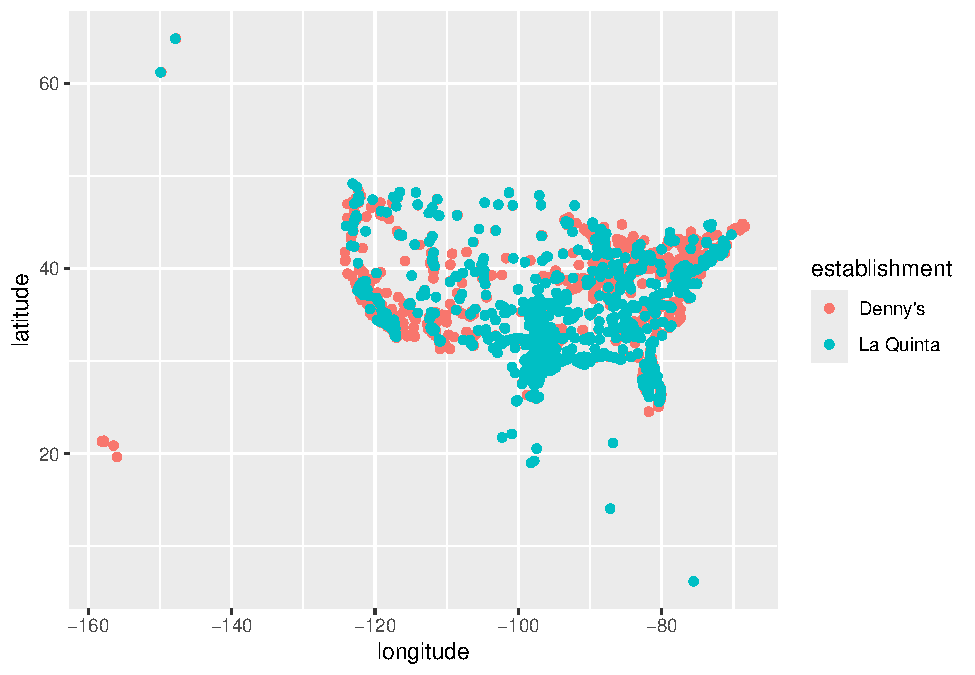
\includegraphics[keepaspectratio]{lab-04-viz-sp-data_files/figure-latex/unnamed-chunk-9-1.pdf}}

The following two questions ask you to create visualizations. These
should follow best practices you learned in class, such as informative
titles, axis labels, etc. See
\url{http://ggplot2.tidyverse.org/reference/labs.html} for help with the
syntax. You can also choose different themes to change the overall look
of your plots, see
\url{http://ggplot2.tidyverse.org/reference/ggtheme.html} for help with
these.

\begin{Shaded}
\begin{Highlighting}[]
\CommentTok{\# Denny\textquotesingle{}s per thousand square miles}
\NormalTok{dennys\_per\_area }\OtherTok{\textless{}{-}}\NormalTok{ dennys }\SpecialCharTok{\%\textgreater{}\%}
  \FunctionTok{count}\NormalTok{(state) }\SpecialCharTok{\%\textgreater{}\%}
  \FunctionTok{inner\_join}\NormalTok{(states, }\AttributeTok{by =} \FunctionTok{c}\NormalTok{(}\StringTok{"state"} \OtherTok{=} \StringTok{"abbreviation"}\NormalTok{)) }\SpecialCharTok{\%\textgreater{}\%}
  \FunctionTok{mutate}\NormalTok{(}\AttributeTok{locations\_per\_1000sqmi =}\NormalTok{ n }\SpecialCharTok{/}\NormalTok{ (area }\SpecialCharTok{/} \DecValTok{1000}\NormalTok{)) }\SpecialCharTok{\%\textgreater{}\%}
  \FunctionTok{arrange}\NormalTok{(}\FunctionTok{desc}\NormalTok{(locations\_per\_1000sqmi))}

\CommentTok{\# Top 5 states by Denny\textquotesingle{}s density}
\FunctionTok{cat}\NormalTok{(}\StringTok{"Top 5 states by Denny\textquotesingle{}s per 1000 square miles:}\SpecialCharTok{\textbackslash{}n}\StringTok{"}\NormalTok{)}
\end{Highlighting}
\end{Shaded}

\begin{verbatim}
## Top 5 states by Denny's per 1000 square miles:
\end{verbatim}

\begin{Shaded}
\begin{Highlighting}[]
\FunctionTok{head}\NormalTok{(dennys\_per\_area }\SpecialCharTok{\%\textgreater{}\%} \FunctionTok{select}\NormalTok{(state, n, area, locations\_per\_1000sqmi), }\DecValTok{5}\NormalTok{)}
\end{Highlighting}
\end{Shaded}

\begin{verbatim}
## # A tibble: 5 x 4
##   state     n     area locations_per_1000sqmi
##   <chr> <int>    <dbl>                  <dbl>
## 1 DC        2     68.3                  29.3 
## 2 RI        5   1545.                    3.24
## 3 CA      403 163695.                    2.46
## 4 CT       12   5543.                    2.16
## 5 FL      140  65758.                    2.13
\end{verbatim}

\begin{Shaded}
\begin{Highlighting}[]
\CommentTok{\# La Quinta per thousand square miles}
\NormalTok{laquinta\_per\_area }\OtherTok{\textless{}{-}}\NormalTok{ laquinta }\SpecialCharTok{\%\textgreater{}\%}
  \FunctionTok{filter}\NormalTok{(country }\SpecialCharTok{==} \StringTok{"United States"}\NormalTok{) }\SpecialCharTok{\%\textgreater{}\%}
  \FunctionTok{count}\NormalTok{(state) }\SpecialCharTok{\%\textgreater{}\%}
  \FunctionTok{inner\_join}\NormalTok{(states, }\AttributeTok{by =} \FunctionTok{c}\NormalTok{(}\StringTok{"state"} \OtherTok{=} \StringTok{"abbreviation"}\NormalTok{)) }\SpecialCharTok{\%\textgreater{}\%}
  \FunctionTok{mutate}\NormalTok{(}\AttributeTok{locations\_per\_1000sqmi =}\NormalTok{ n }\SpecialCharTok{/}\NormalTok{ (area }\SpecialCharTok{/} \DecValTok{1000}\NormalTok{)) }\SpecialCharTok{\%\textgreater{}\%}
  \FunctionTok{arrange}\NormalTok{(}\FunctionTok{desc}\NormalTok{(locations\_per\_1000sqmi))}

\CommentTok{\# Top 5 states by La Quinta density}
\FunctionTok{cat}\NormalTok{(}\StringTok{"Top 5 states by La Quinta per 1000 square miles:}\SpecialCharTok{\textbackslash{}n}\StringTok{"}\NormalTok{)}
\end{Highlighting}
\end{Shaded}

\begin{verbatim}
## Top 5 states by La Quinta per 1000 square miles:
\end{verbatim}

\begin{Shaded}
\begin{Highlighting}[]
\FunctionTok{head}\NormalTok{(laquinta\_per\_area }\SpecialCharTok{\%\textgreater{}\%} \FunctionTok{select}\NormalTok{(state, n, area, locations\_per\_1000sqmi), }\DecValTok{5}\NormalTok{)}
\end{Highlighting}
\end{Shaded}

\begin{verbatim}
## # A tibble: 5 x 4
##   state     n    area locations_per_1000sqmi
##   <chr> <int>   <dbl>                  <dbl>
## 1 RI        2   1545.                  1.29 
## 2 FL       74  65758.                  1.13 
## 3 CT        6   5543.                  1.08 
## 4 MD       13  12406.                  1.05 
## 5 TX      237 268596.                  0.882
\end{verbatim}

Rhode Island and DC have high densities due to their small areas.
Adjusting for area gives us a different perspective on concentration.

\begin{enumerate}
\def\labelenumi{\arabic{enumi}.}
\setcounter{enumi}{10}
\tightlist
\item
  Filter the data for observations in North Carolina only, and recreate
  the plot. You should also adjust the transparency of the points, by
  setting the \texttt{alpha} level, so that it's easier to see the
  overplotted ones. Visually, does Mitch Hedberg's joke appear to hold
  here?
\end{enumerate}

\begin{Shaded}
\begin{Highlighting}[]
\NormalTok{dn\_lq }\SpecialCharTok{\%\textgreater{}\%}
  \FunctionTok{filter}\NormalTok{(state }\SpecialCharTok{==} \StringTok{"NC"}\NormalTok{) }\SpecialCharTok{\%\textgreater{}\%}
  \FunctionTok{ggplot}\NormalTok{(}\AttributeTok{mapping =} \FunctionTok{aes}\NormalTok{(}\AttributeTok{x =}\NormalTok{ longitude, }\AttributeTok{y =}\NormalTok{ latitude, }\AttributeTok{color =}\NormalTok{ establishment)) }\SpecialCharTok{+}
  \FunctionTok{geom\_point}\NormalTok{(}\AttributeTok{alpha =} \FloatTok{0.7}\NormalTok{, }\AttributeTok{size =} \DecValTok{2}\NormalTok{) }\SpecialCharTok{+}
  \FunctionTok{labs}\NormalTok{(}
    \AttributeTok{title =} \StringTok{"Denny\textquotesingle{}s and La Quinta Locations in North Carolina"}\NormalTok{,}
    \AttributeTok{x =} \StringTok{"Longitude"}\NormalTok{,}
    \AttributeTok{y =} \StringTok{"Latitude"}\NormalTok{,}
    \AttributeTok{color =} \StringTok{"Establishment"}
\NormalTok{  ) }\SpecialCharTok{+}
  \FunctionTok{theme\_minimal}\NormalTok{() }\SpecialCharTok{+}
  \FunctionTok{coord\_quickmap}\NormalTok{()  }\CommentTok{\# Alternative that doesn\textquotesingle{}t require mapproj}
\end{Highlighting}
\end{Shaded}

\pandocbounded{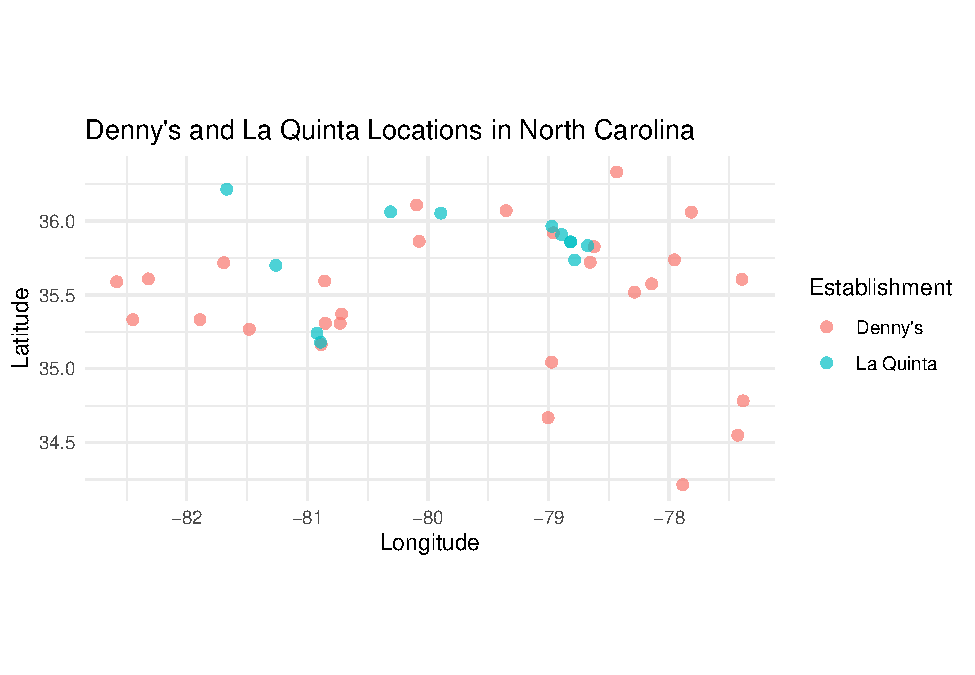
\includegraphics[keepaspectratio]{lab-04-viz-sp-data_files/figure-latex/nc-plot-1.pdf}}

Looking at the North Carolina plot, there does appear to be some
clustering of Denny's and La Quinta locations, particularly around major
cities and along interstate corridors. However, the pattern isn't
overwhelming - there are many Denny's without nearby La Quintas and vice
versa. The joke partially holds but isn't a universal truth.

\begin{enumerate}
\def\labelenumi{\arabic{enumi}.}
\setcounter{enumi}{11}
\tightlist
\item
  Now filter the data for observations in Texas only, and recreate the
  plot, with an appropriate \texttt{alpha} level. Visually, does Mitch
  Hedberg's joke appear to hold here?
\end{enumerate}

\begin{Shaded}
\begin{Highlighting}[]
\NormalTok{dn\_lq }\SpecialCharTok{\%\textgreater{}\%}
  \FunctionTok{filter}\NormalTok{(state }\SpecialCharTok{==} \StringTok{"TX"}\NormalTok{) }\SpecialCharTok{\%\textgreater{}\%}
  \FunctionTok{ggplot}\NormalTok{(}\AttributeTok{mapping =} \FunctionTok{aes}\NormalTok{(}\AttributeTok{x =}\NormalTok{ longitude, }\AttributeTok{y =}\NormalTok{ latitude, }\AttributeTok{color =}\NormalTok{ establishment)) }\SpecialCharTok{+}
  \FunctionTok{geom\_point}\NormalTok{(}\AttributeTok{alpha =} \FloatTok{0.5}\NormalTok{, }\AttributeTok{size =} \FloatTok{1.5}\NormalTok{) }\SpecialCharTok{+}
  \FunctionTok{labs}\NormalTok{(}
    \AttributeTok{title =} \StringTok{"Denny\textquotesingle{}s and La Quinta Locations in Texas"}\NormalTok{,}
    \AttributeTok{x =} \StringTok{"Longitude"}\NormalTok{, }
    \AttributeTok{y =} \StringTok{"Latitude"}\NormalTok{,}
    \AttributeTok{color =} \StringTok{"Establishment"}
\NormalTok{  ) }\SpecialCharTok{+}
  \FunctionTok{theme\_minimal}\NormalTok{() }\SpecialCharTok{+}
  \FunctionTok{coord\_quickmap}\NormalTok{() }\SpecialCharTok{+}  \CommentTok{\# Alternative that doesn\textquotesingle{}t require mapproj}
  \FunctionTok{scale\_color\_manual}\NormalTok{(}\AttributeTok{values =} \FunctionTok{c}\NormalTok{(}\StringTok{"Denny\textquotesingle{}s"} \OtherTok{=} \StringTok{"\#FF6B6B"}\NormalTok{, }\StringTok{"La Quinta"} \OtherTok{=} \StringTok{"\#4ECDC4"}\NormalTok{))}
\end{Highlighting}
\end{Shaded}

\pandocbounded{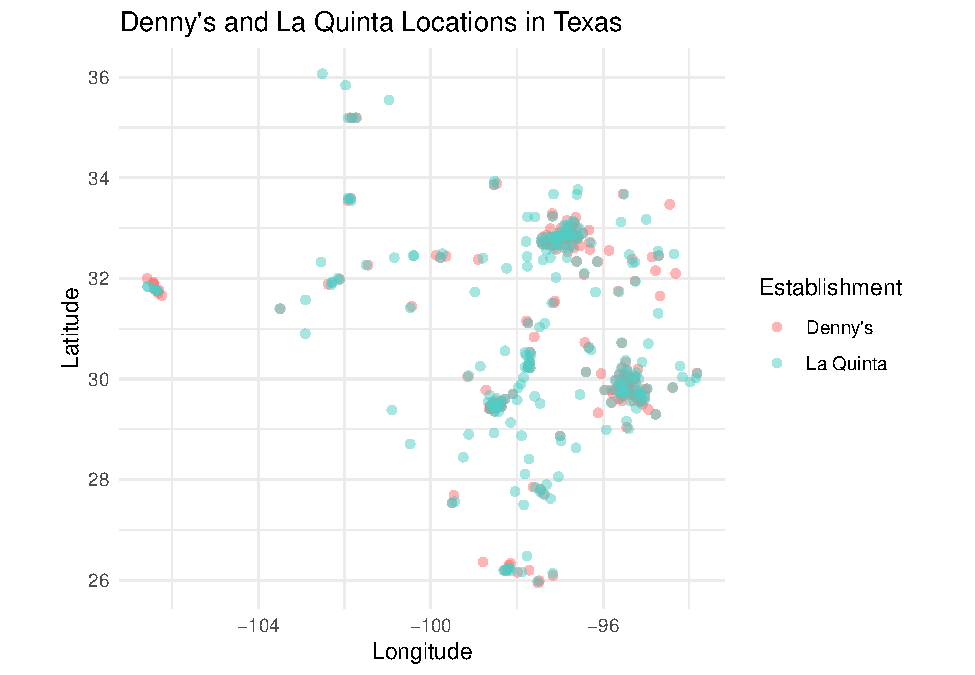
\includegraphics[keepaspectratio]{lab-04-viz-sp-data_files/figure-latex/tx-plot-1.pdf}}

In Texas, with many more locations of both establishments, we can see
some clustering patterns, especially in major metropolitan areas like
Houston, Dallas, Austin, and San Antonio. There does appear to be some
tendency for the two chains to locate near each other, particularly
along major highways. However, there are also many locations of each
chain that are not near the other. The joke seems to have some basis in
reality but is an exaggeration.

That's it for now! In the next lab we will take a more quantitative
approach to answering these questions.

🧶 ✅ ⬆️ Knit, \emph{commit, and push your changes to GitHub with an
appropriate commit message. Make sure to commit and push all changed
files so that your Git pane is cleared up afterwards and review the md
document on GitHub to make sure you're happy with the final state of
your work.}

Now go back through your write up to make sure you've answered all
questions and all of your R chunks are properly labeled. Once you decide
that you are done with the lab, choose the knit drop down and select
\texttt{Knit\ to\ tufte\_handout} to generate a pdf. Download and submit
that pdf to Canvas.

\end{document}
